\section{\label{sec:scale}Scaling Analysis}
The Gung Ho dynamical core uses an unstructured mesh to avoid a
singular pole which ultimately inhibits the scaling of the
UM. Examining the scaling behavour of the model to if the model can
perform sufficiently well is therefore important. To test the scaling a series
of model runs was performed. The version of the LFRic repository trunk
was $17483$. The code was compiled on the XCS with the Intel 17
compiler, at production level which is \verb+-O3+. The baroclinic wave
test was run on a $C576$ mesh. This roughly corresponds to a $17$km
horizontal resolution. The model was run with a $30$km lid and with
$30$ levels.  The time-step used was $180$s
seconds and the benchmarks were run for $100$ time-steps. The code was
profiled using the CrayPAT tool in sampling mode. 

\begin{figure}
\centering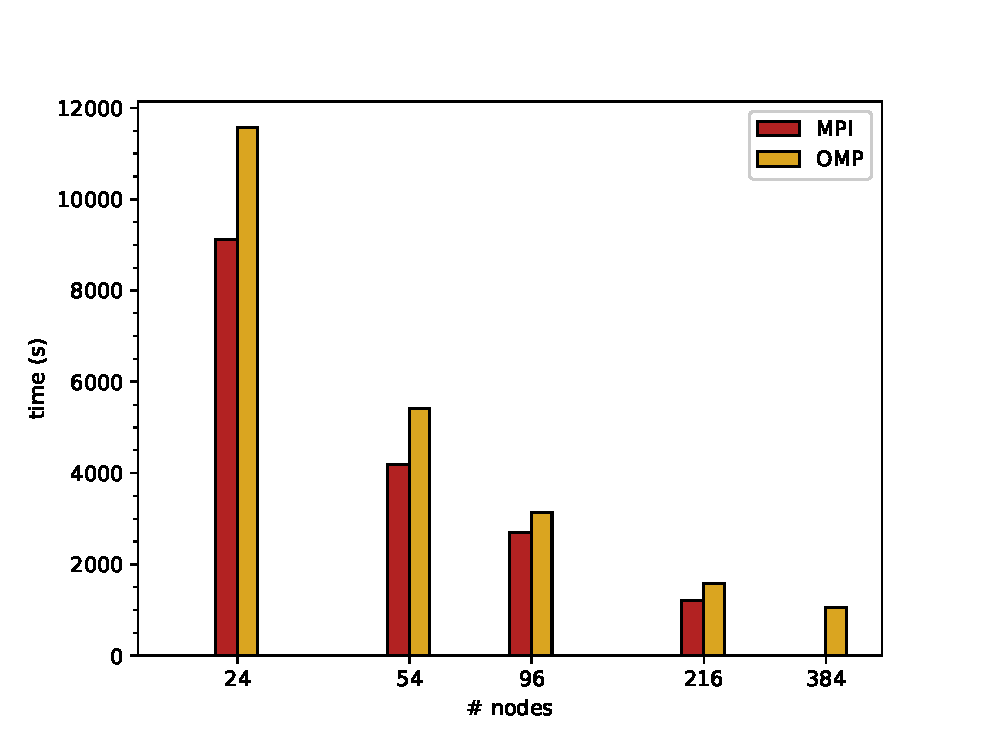
\includegraphics[width=1.0\linewidth]{figs/wc-scale.eps}
\caption{\label{fig:wc_scale}Wall-clock time strong scaling of the 
  Baroclinic wave test. In red, labelled MPI is an MPI only
  version. In yellow, labelled OMP is the hybrid MPI+OpenMP version.}
\end{figure} 

Shown in figure~\ref{fig:wc_scale} is the strong scaling of the whole
model up to $384$ nodes. The MPI only version ran with $36$ MPI ranks
per node. The hybrid version ran with $6$ MPI ranks per node and $6$
openMP threads per MPI rank. The MPI only version on $384$ nodes
crashed during the partitioning phase with an Out Of Memory (OOM)
error. The global mesh is read in by every MPI rank and then
partitioned. This can cause memory problems for large meshes on larger
node counts. This can be solved by a single rank per node reading in
the mesh and broadcasting the partition. The $24$ node hybrid job ran
out of time after 3 hours at $93$ time-steps, so the run time has been
estimated from the log data. This data is also shown in
table~\ref{tab:scale-data}.

\begin{table}
\centering
\caption{\label{tab:scale-data}Wall-clock time of execution of the whole code (WC), User
  code (U), Halo Exchange (HE) and Global Sum (GS) in seconds. Also
  shown is the Local Volume per MPI ranks (LV) and the Halo Size (HS)
  measured in number of horizontal cells.}
\begin{tabular}{r|rrrr|cr}
N & WC & U & HE & GS & LV & HS  \\
    & \multicolumn{4}{c|}{time (s)} & \multicolumn{2}{c}{cells} \\ \hline\hline
     &  \multicolumn{4}{c|}{MPI}& \\
$24$  & $9126$ & $4107$ & $788$ & $502$ & $48\times 48$ & $196$ \\
$54$  & $4196$ & $3139$ & $411$ & $470$ & $32\times 32$ & $132$ \\ 
$96$  & $2693$ & $1508$ & $380$ & $679$ & $24\times 32$ & $100$ \\ 
$216$ & $1202$ & $566$  & $302$ & $174$ & $16\times 16$ & $68$  \\ 
$384$ & $--$   & $--$   & $--$  & $--$  & $12\times 12$ & $54$ \\\hline
  & \multicolumn{4}{c|}{Hybrid} & \\
$24$ &$11566$ & $--$    & $--$  & $--$ & $96\times 144$ & $484$ \\
$54$ & $5410$  & $2732$ & $1282$ & $887$ & $64\times 96$ & $324$ \\
$96$ &$3140$  & $1332$ & $895$ & $562$ & $48\times 72$ & $244$ \\
$216$ &$1585$  & $468$ & $485$ & $384$ & $32\times 48$ & $164$ \\
$384$ &$1059$  & $222$ & $310$ & $322$ & $24\times 32$ & $124$ \\\hline
\end{tabular}
\end{table}

The model shows good scaling for both the MPI and hybrid programming
models. The parallel efficiency is reasonable, the $216$ node job uses
$9\times $ the resouces of the $24$ node job and both the MPI and
hybrid version run more than $7\times $ faster . The hybrid code for the
$384$ node job which has $16\times $ the resource of the $24$ node
job, runs approxmiately $11 \times$ faster.

Compared to the scaling runs performed with the {\em Fallow Deer} (FD)
release of LFRic and reported in~\cite{lfric} there is an apparent
change in the OpenMP behaviour. The FD scaling shows the hybrid version of
the code is faster than the MPI version, whereas the opposite is now
true for the data displayed here. 

\begin{figure}
\centering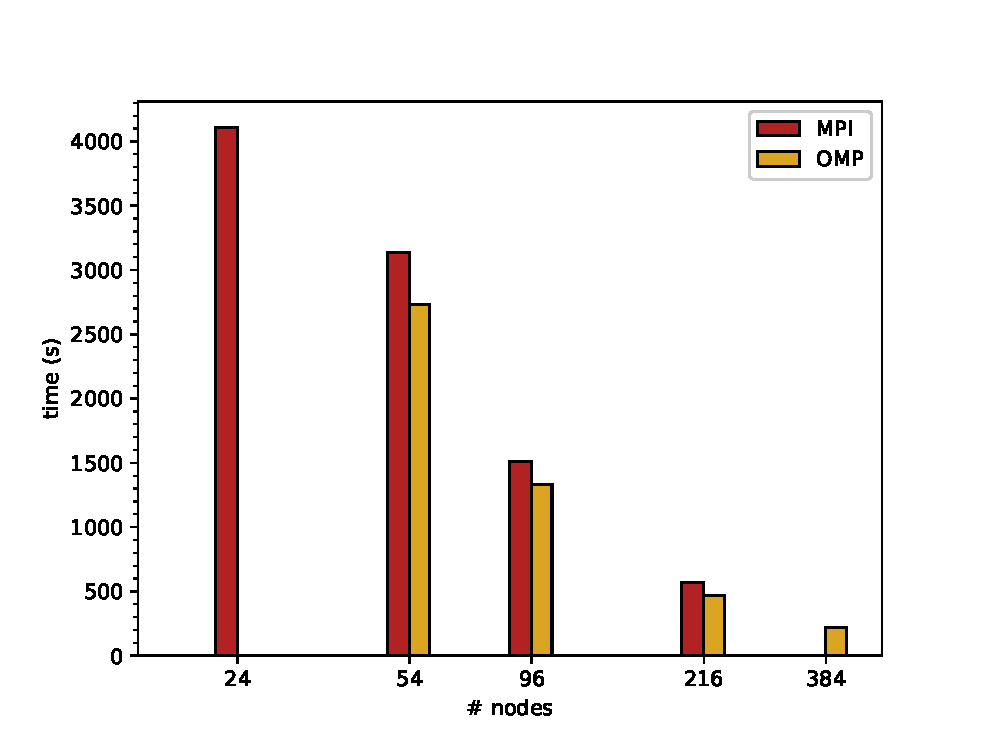
\includegraphics[width=1.0\linewidth]{figs/U-scale.eps}
\caption{\label{fig:U_scale}Wall-clock time strong scaling of the 
  User code from Baroclinic wave test.}
\end{figure} 

\begin{figure}
\centering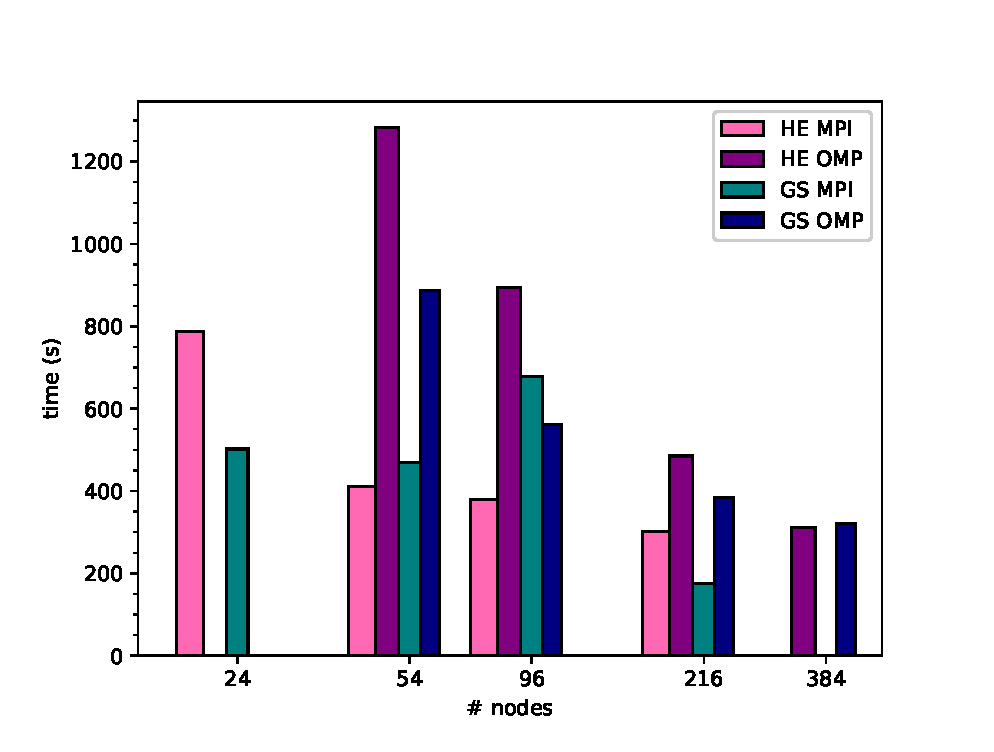
\includegraphics[width=1.0\linewidth]{figs/comms-scale.eps}
\caption{\label{fig:comns_scale}Wall-clock time strong scaling of the 
  communications costs of the Baroclinic wave test.}
\end{figure} 

